% Autor: Leonhard Segger, Alexander Neuwirth
% Datum: 2017-10-30
\documentclass[
	% Papierformat
	a4paper,
	% Schriftgröße (beliebige Größen mit „fontsize=Xpt“)
	12pt,
	% Schreibt die Papiergröße korrekt ins Ausgabedokument
	pagesize,
	% Sprache für z.B. Babel
	ngerman
]{scrartcl}

% Achtung: Die Reihenfolge der Pakete kann (leider) wichtig sein!
% Insbesondere sollten (so wie hier) babel, fontenc und inputenc (in dieser
% Reihenfolge) als Erstes und hyperref und cleveref (Reihenfolge auch hier
% beachten) als Letztes geladen werden!

% Silbentrennung etc.; Sprache wird durch Option bei \documentclass festgelegt
\usepackage{babel}
% Verwendung der Zeichentabelle T1 (Sonderzeichen etc.)
\usepackage[T1]{fontenc}
% Legt die Zeichenkodierung der Eingabedatei fest, z.B. UTF-8
\usepackage[utf8]{inputenc}
% Schriftart
\usepackage{lmodern}
% Zusätzliche Sonderzeichen
\usepackage{textcomp}

% Mathepaket (intlimits: Grenzen über/unter Integralzeichen)
\usepackage[intlimits]{amsmath}
% Ermöglicht die Nutzung von \SI{Zahl}{Einheit} u.a.
\usepackage{siunitx}
% Zum flexiblen Einbinden von Grafiken (\includegraphics)
\usepackage{graphicx}
% Abbildungen im Fließtext
\usepackage{wrapfig}
% Abbildungen nebeneinander (subfigure, subtable)
\usepackage{subcaption}
% Funktionen für Anführungszeichen
\usepackage{csquotes}
% Zitieren, Bibliographie
\usepackage{biblatex}


% Zur Darstellung von Webadressen
\usepackage{url}
%chemische Formeln
\usepackage[version=4]{mhchem}
% siunitx: Deutsche Ausgabe, Messfehler getrennt mit ± ausgeben
\usepackage{floatrow}
\floatsetup[table]{capposition=top}
\usepackage{float}
% Verlinkt Textstellen im PDF-Dokument
\usepackage[unicode]{hyperref}
% "Schlaue" Referenzen (nach hyperref laden!)
\usepackage{cleveref}
\sisetup{
	locale=DE,
	separate-uncertainty
}
%\bibliography{6Mi_M3_29-11-2017_References}
%TODO anpassen

\begin{document}
	
	\begin{titlepage}
		\centering
		{\scshape\LARGE Versuchsbericht zu \par}
		\vspace{1cm}
		{\scshape\huge A3 - Absorption von Beta- und Gamma-Strahlung \par}
		\vspace{2.5cm}
		{\LARGE Gruppe 14Mo \par}
		\vspace{0.5cm}
		
		{\large Alexander Neuwirth (E-Mail: a\_neuw01@wwu.de) \par}
		{\large Leonhard Segger (E-Mail: l\_segg03@uni-muenster.de) \par}
		\vfill
		
		durchgeführt am 07.05.2018\par
		betreut von\par
		{\large Johann Preuß}  
		
		\vfill
		
		{\large \today\par}
	\end{titlepage}
	\tableofcontents
	\newpage

	\section{Kurzfassung}
	%TODO Hypothese	und deren Ergebnis, wenn Hypothese ist, dass nur Theorie erfüllt, sagen: Erwartung: Theorie aus einführung (mit reflink) erfüllt
	%TODO Ergebnisse, auch Zahlen, mindestens wenn's halbwegs Sinn ergibt
	%TODO Was wurde gemacht
	%TODO manche leute wollen Passiv oder "man", manche nicht
	In diesem Versuch wurde die Absorption von Beta- und Gammastrahlung untersucht. %überflüssig?
	Dazu wurde der Zusammenhang zwischen Schichtdicke eines Absorbers, Art der Strahlung des Präparats und Impulsrate betrachtet.
	
	\section{Methoden}\label{Methoden}
	%TODO Bilder von der Website klauen
	Der Versuchsaufbau bestand aus einem Geiger-Müller-Zählrohr, das an ein Betriebsgerät angeschlossen war.
	Vor das Glimmerfenster des Zählrohrs konnten nun verschiedene radioaktive Präparate installiert werden und unterschiedliche Absorber zwischen Präparat und Röhre gebracht werden.
	
	Zunächst wurde die Zählrohrcharakteristik des Geiger-Müller-Zählrohres bestimmt, um die folgenden Untersuchungen im Plateaubereich der Zählrohrkennlinie durchführen zu können.
	Dazu wurde die Impulsrate des Zählrohrs mit $\beta$-Präparat bei steigender Zählrohrspannung bestimmt.
	Begonnen wurde hier unmittelbar unter der Einsatzspannung und die folgenden Messungen wurden bei ca. \SI{100}{\volt} über der Einsatzspannung durchgeführt.
	
	Dann wurde, um die mittlere Untergrundaktivität zu bestimmen, 200 mal die Zahl der Untergrundimpulse in \SI{10}{\second} gemessen.
	Anschließend wurde die Impulsrate des $\gamma$-Präparats mit zunehmender Schichtdicke des Blei-Absorbers gemessen und die Impulsrate des $\beta$-Präparats mit zunehmender Aluminium-Absorber-Dicke.
	Zuletzt wurde noch die Impulsrate des $\beta$-Präparats mit Plexiglas- und Gummiabsorber bei konstanter Schichtdicke bestimmt.
	
	Hierbei wurden jeweils mindestens 1111 Impulse gemessen, um die relative Unsicherheit unter 3\% zu halten.
	Die Betriebsspannung wurde vom Betriebsgerät abgelesen und nich mit einem externen Voltmeter überprüft.
	
	%TODO Bestimmen der Zählzeit => 1111 Impulse
	%TODO Einstellrad für Spannung => keine überprüfung mit voltmeter ggf erwähn
	
	\section{Ergebnisse und Diskussion}
	%TODO Datenanalyse -> Überschrift?
	%TODO Unsicherheiten
	

	\subsection{Beobachtung}
	%TODO Einflüsse von veränderten Parametern auf Messung
	In \cref{Zaehlrohrcharakteristik} ist die Impulsrate gegen die Zählrohrspannung aufgetragen. 
	Es ist ersichtlich, dass die Einsatzspannung zwischen 300 und \SI{325}{V} liegt.
	
	%TODO mehr!
	
	\begin{figure}[H]
		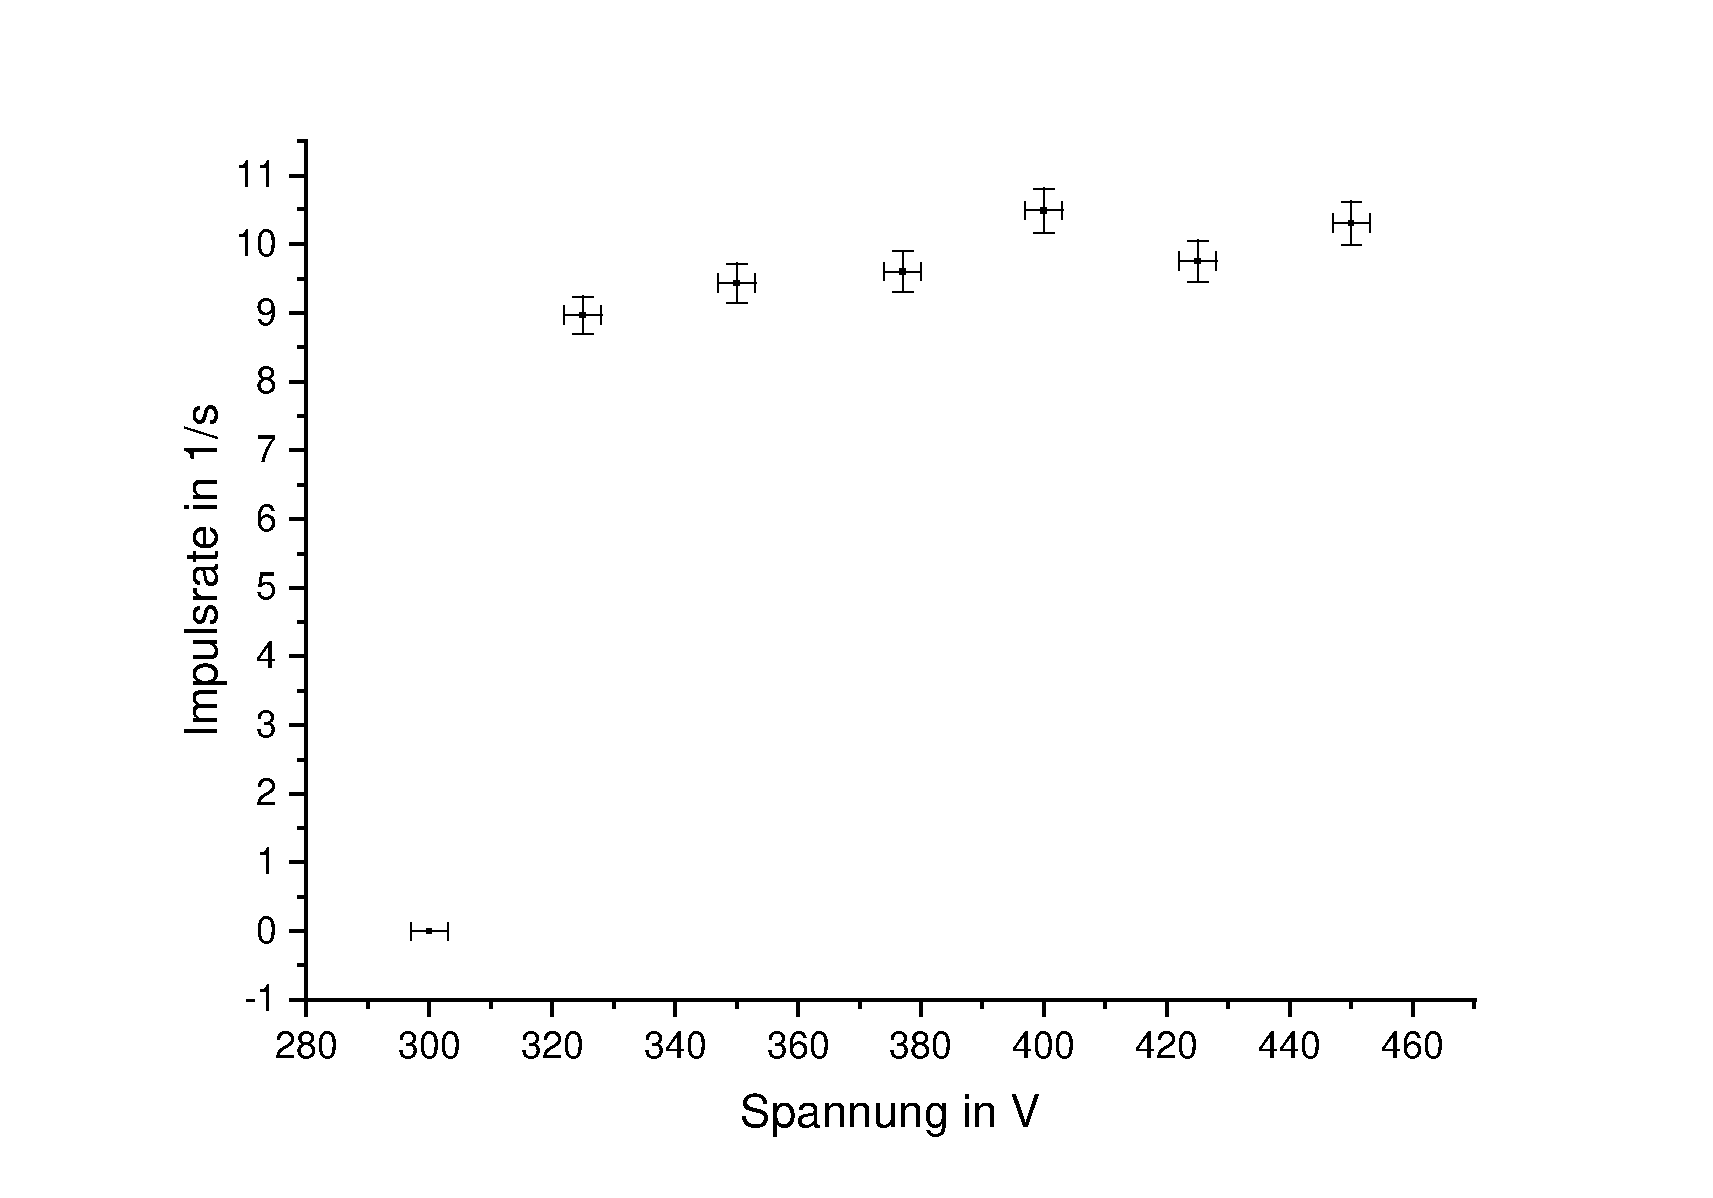
\includegraphics[width=0.7\textwidth]{Zaehlrohrcharakteristik}
		\centering
		\caption{Aufgenommene Zählrohrcharakteristik unter Verwendung eines $\beta$-Präparat.}%TODO Titel
		\label{Zaehlrohrcharakteristik}
		\centering
	\end{figure}

	\subsubsection{Unsicherheiten} %TODO Schon alles?
	Die Unsicherheit der Betriebsspannung des Geiger-Müller-Zahlrohrs beträgt \SI{3}{V} (Dreieckverteilung).  
	Die Zählzeit wurde in Sekunden auf einer Digitalanzeige gestoppt wodurch sich eine Unsicherheit von \SI{0,6}{s} ergibt (Rechteckverteilung).
	Wie in \cref{Methoden} beschrieben ist die relative Unsicherheit der Impulsmessungen kleiner 3\%.
	Die Bestimmung der Breite eines Absorbers hat eine Unsicherheit von \SI{0,12}{mm}, die zusammengesetzt ist aus der Genauigkeit des Messschiebers und dem Fehler durch die ungleichmässige Oberfläche des Materials.
	\subsection{Datenanalyse}
	\subsubsection{Untergrundpulse}
	Die Messung der Untergrundimpulse über 200 mal 10 Sekunden ergab einen Mittelwert von 2,685 Impulsen und eine Standardabweichung von 1,519. 
	In \cref{Untergrund} sind die absolute und relative Häufigkeitsverteilungen dargestellt, da sich die Ordinatenwerte lediglich um einen Faktor von 200 unterscheiden lässt sich an der linken Achse die absolute und an der rechten die relative Häufigkeit ablesen.
	Des Weiteren ist in \cref{Untergrund} die Poisson-Verteilung für $\bar{N}$ = 2,685 abgebildet.
	\begin{equation}
		\psi(N) = \frac{\bar{N}^N \cdot e^{(-\bar{N})}}{N!}
	\label{Poisson}
	\end{equation}
	
	\begin{figure}[H]
		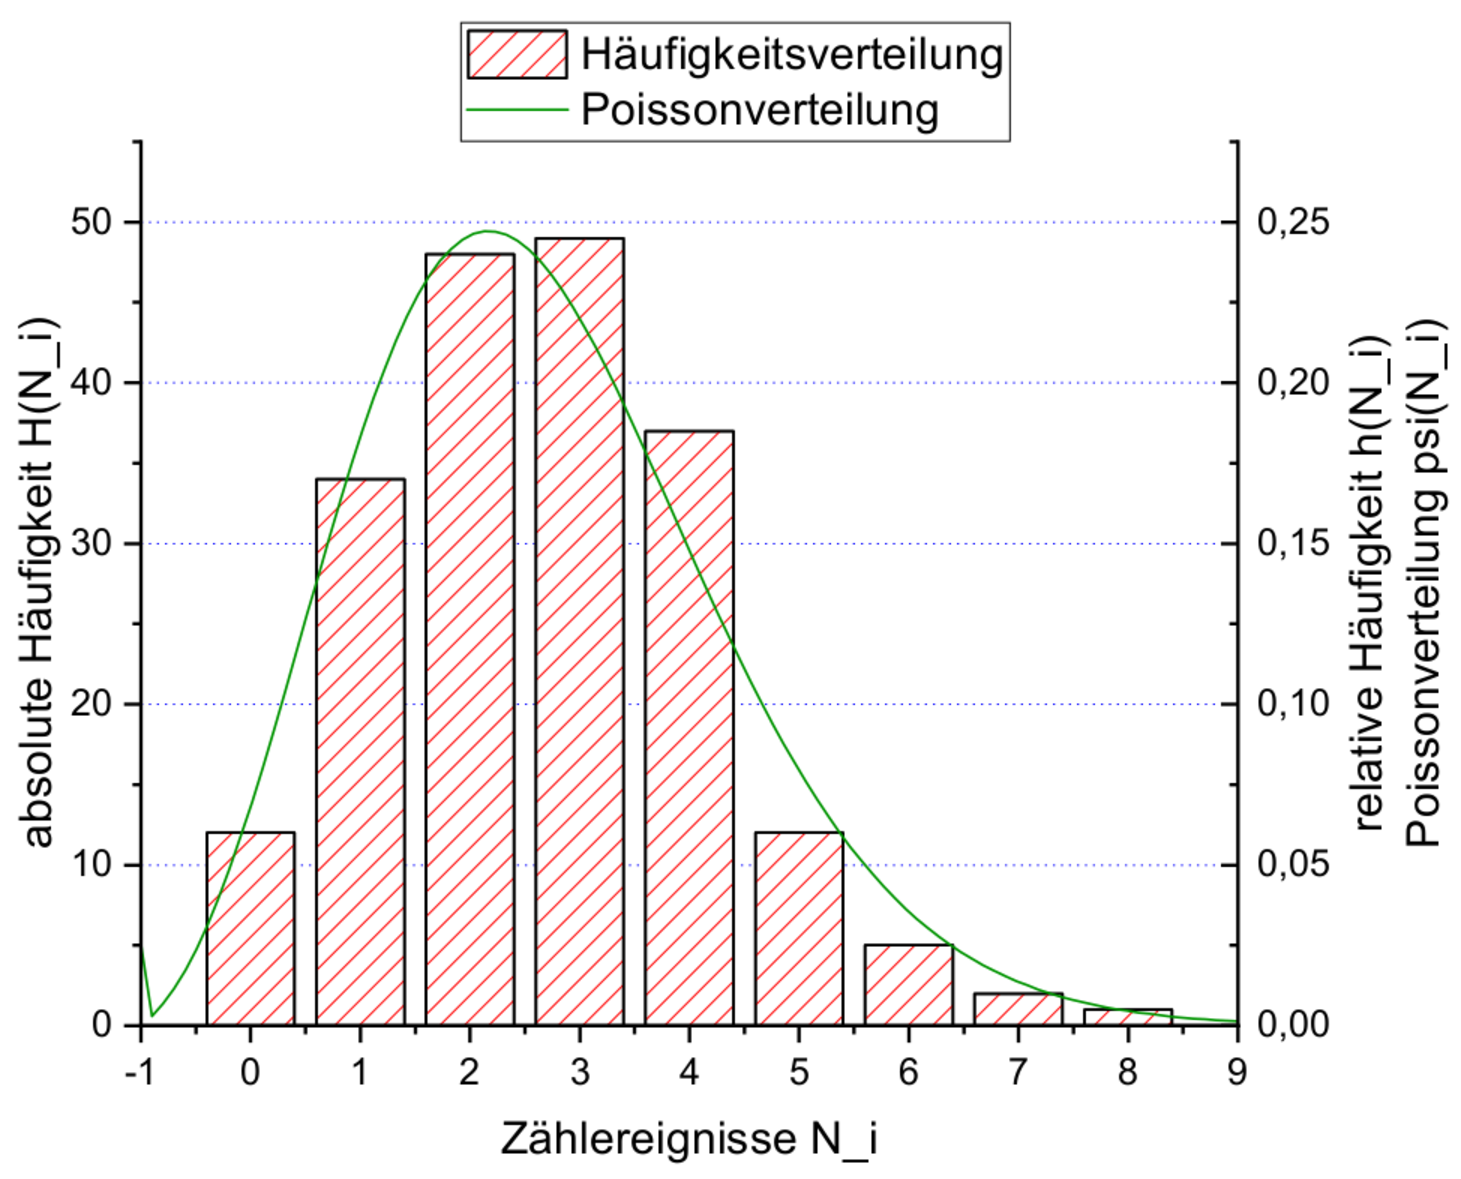
\includegraphics[width=0.7\textwidth]{Untergrund}
		\centering
		\caption{Aufgenommene absolute und relative Häufigkeitsverteilung der Untergrundpulse. Außerdem ist die durch deren Mittelwert festgelegte Poisson-Verteilung abgebildet.}%TODO Titel
		\label{Untergrund}
		\centering
	\end{figure}

	\subsubsection{Absorption von $\gamma$-Strahlung durch Blei} \label{blei}
	In \cref{GammaBlei} ist die Zählrate des $\gamma$-Präparats $ ^{137}$Cs logarithmisch gegen die Breite des Bleis aufgetragen. 
	Von der gemessenen Zählrate wurde die mittlere Untergrundaktivität \SI{0,2685}{Bq} abgezogen.
	Aus der Einführung ist bekannt, dass die Absorption von $\gamma$-Strahlung exponentiell zur Dicke ist,mit:
	\begin{equation}
		a_{\gamma}(x) = a_{\gamma,0} \cdot exp(-\mu_\gamma x)= a_{\gamma,0} \cdot exp(-\mu_{\gamma,m} \rho x)
		\label{gamma}
	\end{equation}
	 Deshalb kann man bei einer logarithmischen Zählrate von einem linaren Zusammenhang zur Breite des Absorbers ausgehen. 
	 Entsprechend ist in \cref{GammaBlei} ein linearer Fit, aus dessen Steigung der Absorptionskoeffizient $\mu_\gamma$ bestimmt werden kann. %TODO cite http://www.chemie.de/lexikon/Blei.html
	 Aus einem $\mu_\gamma$ = $\SI{1,11 +- 0,04}{cm^{-1}}$ und der Dichte von Blei $\rho$ = $\SI{11,34}{g/cm^3}$ folgt ein Masseabsorptionskoeffizient $\mu_{\gamma,m}$ = $\SI{0,0978+-0,0035}{cm^2/g}$.
	 Die Absorptionskoeffizienten hängen von der Strahlungsenergie ab. 
	 Die hier bestimmten $\mu$ wurden bei einer $\gamma$-Strahlung von ca. \SI{0,66}{MeV} gemessen.
	 
	
	
	\begin{figure}[H]
		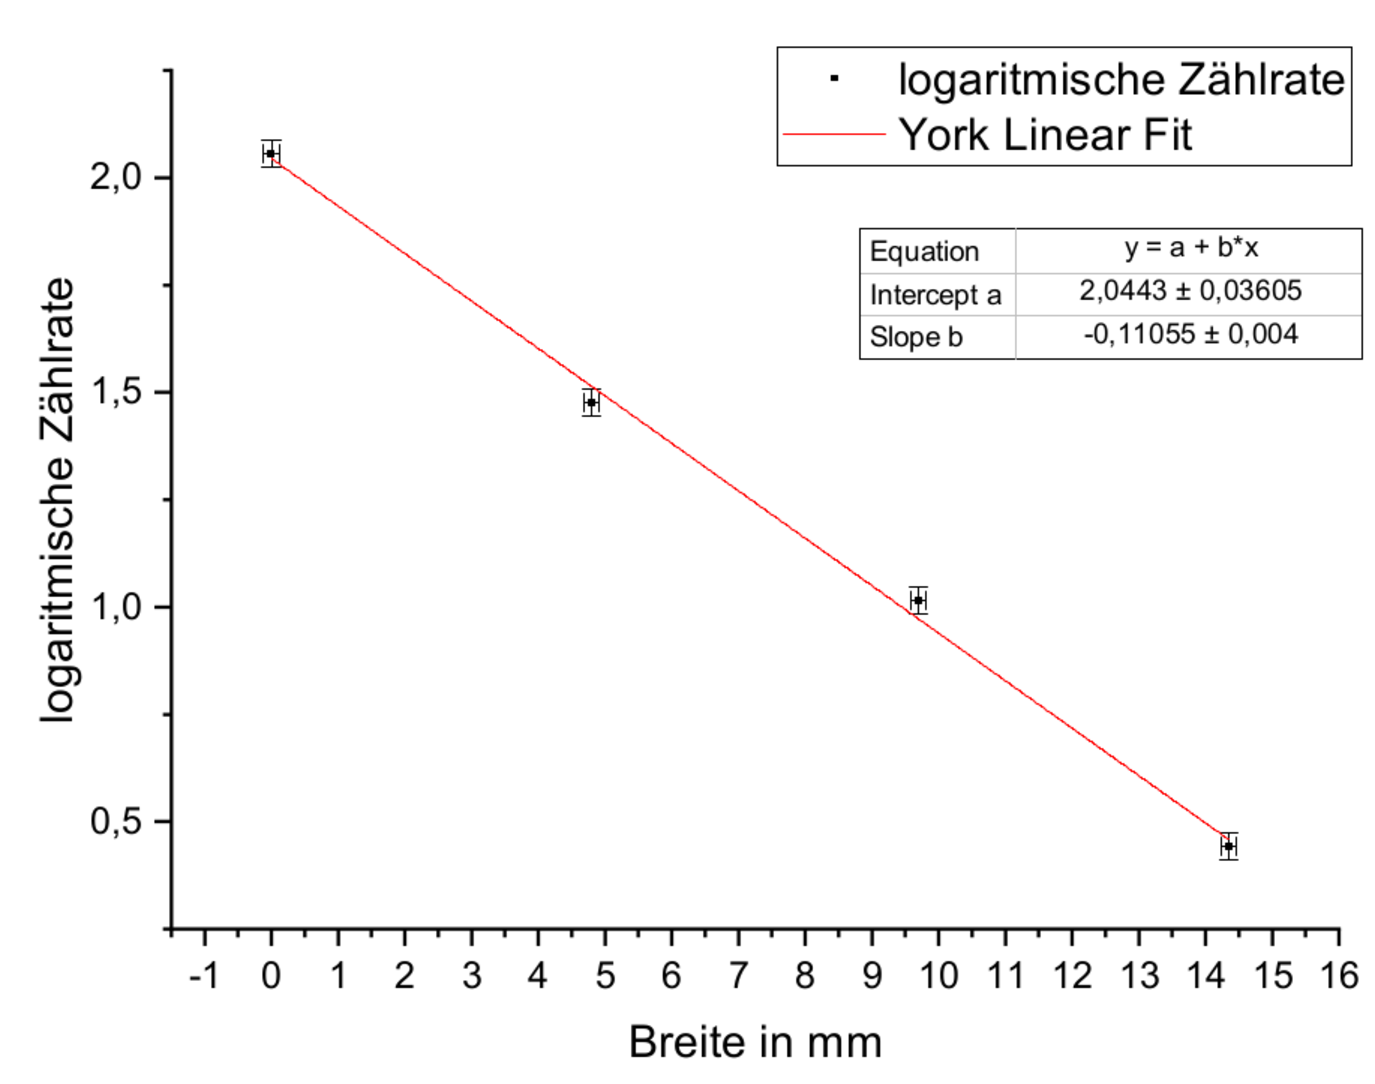
\includegraphics[width=0.7\textwidth]{GammaBlei}
		\centering
		\caption{Die Impulsrate ist logarithmisch gegen die Bleidicke aufgetragen. Als $\gamma$-Präparat wurde $ ^{137}$Cs verwendet.}%TODO Titel
		\label{GammaBlei}
		\centering
	\end{figure}
	
	
	
	\subsubsection{Absorption von $\beta$-Strahlung} 
	Für die folgenden Rechnungen wurde wie in \cref{blei} beschrieben Untergrundkorrektur durchgeführt.
	\subsubsection*{Aluminium}
	Das verwendete $\beta$-Präparat $^{90}$Sr zerfällt mit $E_{\beta,\text{max}}$= \SI{0,55}{MeV} in $^{90}$Y, welches mit $E_{\beta,\text{max}}$ = \SI{2,28}{MeV} in $^{90}$Zr übergeht.%TODO cite einführung
	Die Strahlung beider Zerfälle überlagert sich, jedoch überwiegt der Anteil des Tochternuklids $^{90}$Y, da sich mithilfe der empirische Beuler-Formel die Reichweite der Elektronen abschätzen lässt:
	\begin{equation}
		R_{\beta,\text{max}} \approx \frac{5,71 \cdot E_{\beta,\text{max}} - 1,61}{\rho}
	\end{equation} %TODO cite http://www.chemie.de/lexikon/Blei.html
	Wobei $E_{\beta,\text{max}}$ in MeV und $\rho$ in $\text{kg/m}^3$ einzusetzten sind.
	Mit $E_{\beta,\text{max}}$= \SI{0,55}{MeV} und $\rho$= $\SI{2,7}{g/cm^3}$ folgt eine Maximale Reichweite von ca. \SI{550}{\micro\meter}. 
	
	Analog zu \cref{blei} lassen sich aus \cref{BetaAlu} Absorptions- und Massenabsorptionskoeffizient bestimmen. 
	Die exponentielle Näherung lässt sich auf den gesamten Bereich anwenden, da hier die logarithmische Zählrate linear zur Breite ist.
	Es ergeben sich $\mu_\beta$ = $\SI{19,5 +- 3,1}{cm^{-1}}$ und $\mu_{\beta,m}$ = $\SI{7,2+-1,1}{cm^2/g}$.
	\begin{figure}[H]
		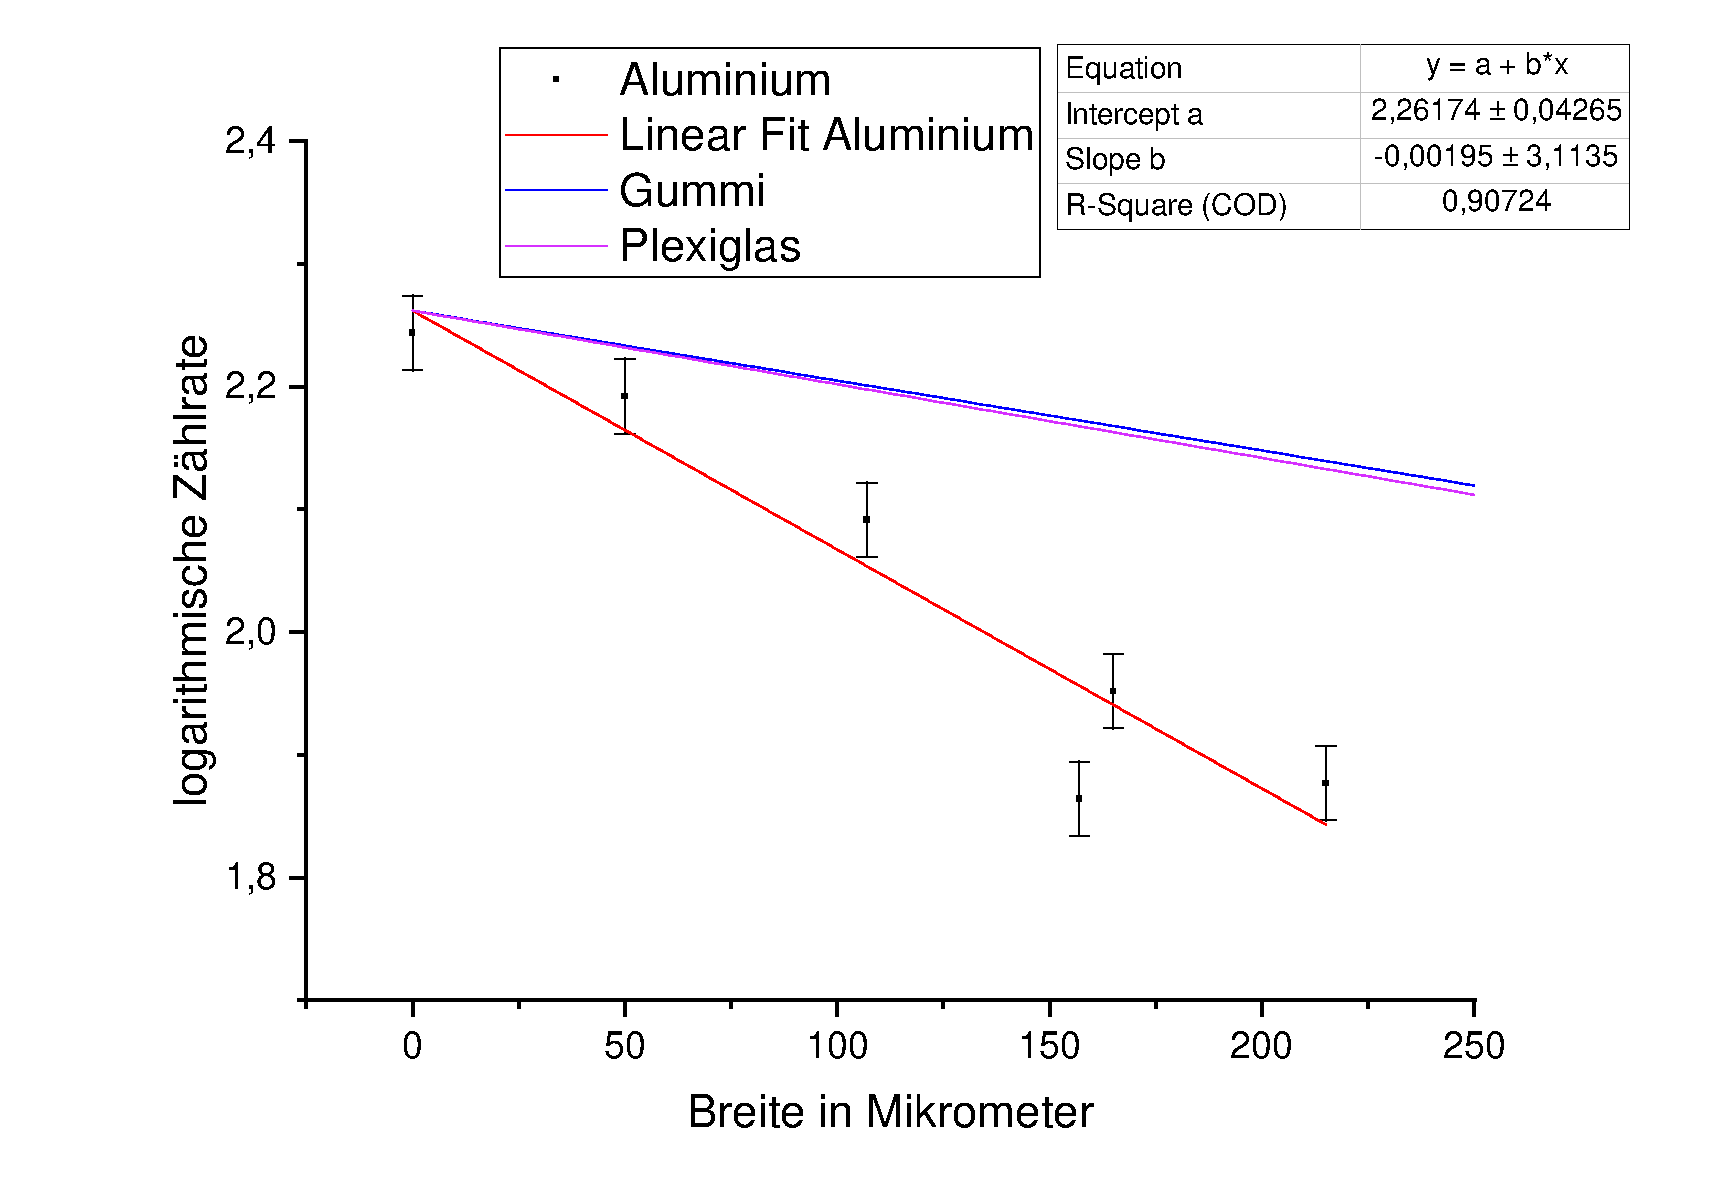
\includegraphics[width=0.7\textwidth]{BetaAlu}
		\centering
		\caption{Die Impulsrate ist logarithmisch gegen die Aluminiumdicke aufgetragen. Als $\beta$-Präparat wurde $ ^{90}$Sr verwendet.}%TODO Titel
		\label{BetaAlu}
		\centering
	\end{figure}	
	
	\subsubsection*{Gummi und Plexiglas} 
	Der Absorptionskoeffizient $\mu_\beta$ lässt sich analog zu $\mu_\gamma$ aus \cref{gamma} durch Umformen bestimmen.
	\begin{equation}
		\mu_\beta = \frac{\ln \left( \frac{a_{\beta,0}}{a_\beta(x)}\right)}{x}
	\end{equation}
	\begin{equation}
	u(\mu_\beta) = \sqrt{ \left(\frac{u(a_{\beta,0})}{a_{\beta,0}x}\right)^2 + \left(\frac{u(a_\beta(x))}{a_\beta(x)x}\right)^2 + \left(\frac{\mu_\beta u(x)}{x}\right)^2}
	\end{equation}
	In \cref{TabelleMu} sind die jeweiligen Parameter von Gummi und Plexiglas sowie das resultierende $\mu_\beta$ aufgeführt.
	Das $a_{\beta,0}$ beträgt \SI{9,43 +- 0,29}{Bq}.
	\begin{table}[H]
		\centering
		\begin{tabular}{ c | c | c }
			&Gummi & Plexiglas \\ \hline
			$x$&\SI{2+-0,12}{mm}&\SI{4+-0,12}{mm}\\
			$a_\beta(x)$&\SI{3,02+-0,09}{Bq}&\SI{0,84+-0,03}{Bq}\\
			$\mu_\beta$&\SI{5,7+-0,4}{cm^{-1}}&\SI{6,0+-0,2}{cm^{-1}}\\
			
		\end{tabular}
		\caption{Aus Breite $x$ und Impulsrate $a_\beta(x)$ berechneter Absorptions- und Masseabsorptionskoeffizient}
		\label{TabelleMu} 
	\end{table}
	
	\subsection{Diskussion}
	%TODO Bezug/Nutzten oder sonst was
	%TODO auch hier die Hypothese wiederholen
	%TODO keine Messwerte hier, nach manchen Menschen, zumindest "direkt" erstellte Diagramme net hier, auch wenn Lesbarkeit-bla
	
	%TODO Poisson passt mit Häufigkeit
	
	
	%TODO Vergleich mu_beta einführungen mit unserem => Energieverteilung
	%TODO ((ggf. Breite > 550 mikrometer besser))
	\section{Schlussfolgerung}
	%TODO Rückgriff auf Hypothese und drittes Nennen dieser
	
	%TODO Quellen zitieren, Websiten mit Zugriffsdatum
	%TODO Verweise auf das Laborbuch (sind erlaubt)
	%TODO Tabelle + Bilder mit Beschriftung
	%\printbibliography
\end{document}
